
\section{The AdEx neuron model}

We choose to simulate the `AdEx' neuron model, or the `adaptive exponential integrate-and-fire' neuron.\cite{Gerstner2009AdaptiveExponentialIntegrateandfire}
This is a leaky-integrate-and-fire (LIF) neuron model, with two additions.
First, the full upstroke of each spike is simulated, as an exponential runoff.
Second, an extra dynamic variable is added: the adaptation current.
This current allows the simulation of many non-linear effects of real neurons, like spike-rate adaptation and post-inhibitory rebound.
% (Note however that we do not focus on adaptation effects in this thesis).

\marginpar{
    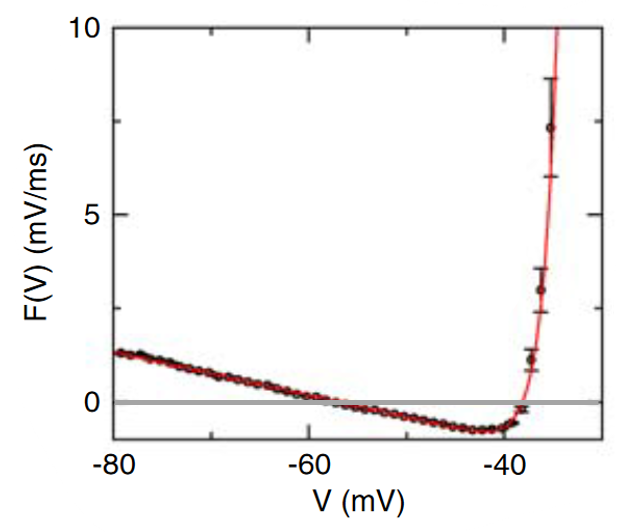
\includegraphics[w=1]{exIF-fit.png}
    \captionof{figure}{A linear-plus-exponential model (red) fit to data from a cortical pyramidal neuron (black), from \cite{Badel2008ExtractingNonlinearIntegrateandfire}}
    \label{fig:exIF-fit}
}

The AdEx model consists of two differential equations, one to simulate the membrane voltage $V$, and one for the adaptation current $w$:
\begin{align}
    C \d{V} &=  -g_L (V - E_L)
                            + g_L Δ_T \exp \left(\frac{V-V_T}{Δ_T}  \right)
                            - I_\syn - w
                            \label{eq:AdEx-V}
                            \\[1em]
    τ_w \d{w} &= a (V - E_L) - w
        \label{eq:AdEx-w}
\end{align}

$I_\syn$ is the synaptic current, explained in \cref{sec:synapse_model}.
We use the sign convention of inter alia Dayan \& Abbott\footnote{\cite{Dayan2001TheoreticalNeuroscienceComputational}, ch.~5.3, p.~162} where membrane currents are defined as positive when positive charges flow \emph{out} of the cell. I.e. a positive $I_\syn$ decreases the membrane voltage (itself defined as the electric potential inside minus outside the cell).

Other parameters are explained in \cref{tab:AdEx-params}.

In this chapter, we will often analyse $\d{V}$ as a function of $V$, i.e. analyse it as a dynamical system: will the voltage increase or decrease at the current voltage?
For conciceness, we will call this function $F(V)$. I.e. $F(V) = \d{V} =$ the right-hand-side of \cref{eq:AdEx-V} here, scaled by $1/ C$. We'll mostly analyse $F$ in the absence of synaptic and adaptation currents, i.e. for $I_\syn$ and $w$ both zero.
\Cref{fig:exIF-fit} shows the $F(V)$ curve for an AdEx neuron fit to a real neuron.

\begin{table}[h]
    \begin{sidecaption}
        {Quantities and parameters of the AdEx neuron, \cref{eq:AdEx-V,eq:AdEx-w,eq:AdEx-reset}. By defining the location of $\d{V}$'s minmum, $V_T$ also determines the location of the firing threshold.}
        [tab:AdEx-params]
        \begin{tabular}{c l l}
            Name  & Description & Units \\
            \hline
            $V$  & Membrane voltage & V \\
            $C$ & Membrane capacitance & F \\
            $g_L$ & Input / leak conductance & S (V/A) \\
            $E_L$  & Resting / leak potential & V \\
            $Δ_T$  & Steepness of $\d{V}$ around the firing threshold & V \\
            $V_T$  & Location of minimum of $\d{V}$ & V \\
            $w$   & Adaptation current & A \\
            $τ_w$   & Time constant of adaptation current & s \\
            $a$ & Sensitivity of adaptation current to $V$ & S \\
        \end{tabular}
    \end{sidecaption}
\end{table}

We solve these equations using first-order (Euler) integration.

In addition to the two differential equations, the AdEx model also consists of an instantaneous reset condition. When the membrane voltage $V$ reaches a certain threshold $θ$, a spike is recorded, $V$ is reset, and $w$ is increased:
\begin{align}
    \text{if}\ V > θ\ \text{then:}\ \label{eq:AdEx-reset}
    & V ← V_r \\
    & w ← w + Δw \notag
\end{align}

% Slowly injecting current $I$ shifts Izhikevich's parabola upwards, raising the resting potential and lowering the spiking threshold. At a certain point, the two fixed points merge and disappear ("annihilate"), in a "saddle--node"\fnm or "fold" bifurcation. The voltage can only go up -- and with the reset of \cref{eq:Izh_V_reset}, the neuron keeps spiking.

% \fnt{In the full $(V, u)$ phase plane, at $V_r$ there is a node (both eigendirections are attracting), and at $V_t$ there is a saddle (only one eigendirection attracts, the other repels). Hence, "saddle--node" bifurcation.}

% On the other hand, negative input currents or a positive adaptation current $u$ shift $\dot{V}$ downwards, giving a lower resting potential and a higher spiking threshold. This is how the model creates spike rate adaptation: every spike increases $u$ (\cref{eq:Izh_u_update}), and thus the spiking threshold.


\subsection{Analysis}

Where are the fixed points of the dynamical system $\d{V} = F(V)$? I.e, where is $F = 0$? Like other neuron models, there are two fixed points: a stable one at the leak potential $E_L$, and an unstable one at the instantaneous firing threshold (which we'll call $E_T$).

We see in \cref{eq:AdEx-V} (for $I_\syn = 0$ and $w = 0$) that the leak potential $E_L$ is indeed a fixed point -- or rather lies very close to one: the exponential term is negligibly small at $V = E_L$.
\marginpar{
    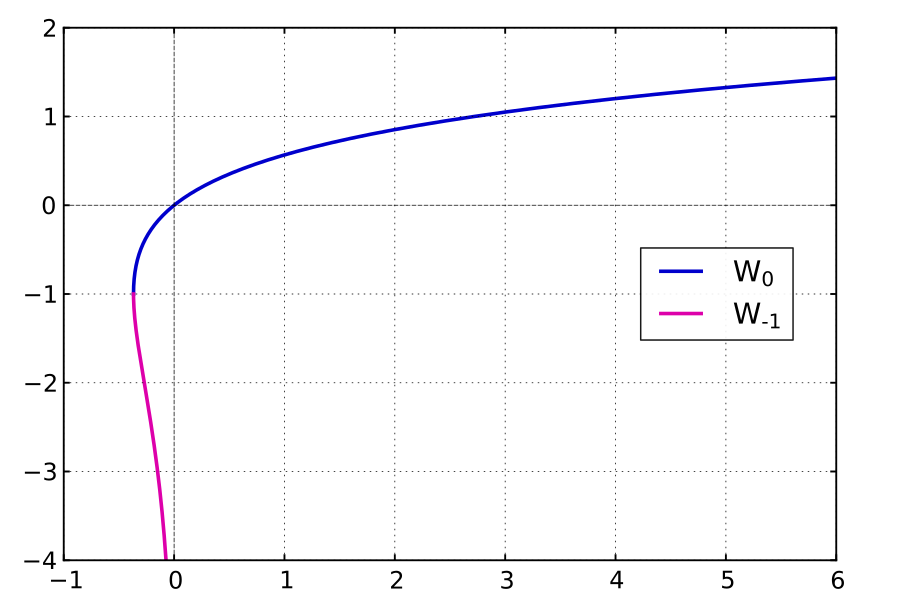
\includegraphics[w=1]{LambertW.png}
    \captionof{figure}{The Lambert $W$ functions for real numbers.}
    \label{fig:LambertW}
}
The second fixed point has no straightforward expression. The exact solutions for $F$'s roots need the so called Lambert $W$ or `product logarithm' functions $W_0$ and $W_{-1}$ (see \cref{fig:LambertW}). The roots are found at:
\begin{equation}
    V = E_L - Δ_T W_k \left( -\exp\left( \frac{E_L - V_T}{Δ_T} \right) \right) \label{eq:LambertW}
\end{equation}
..where $k = 0$ gives the resting potential, and $k = -1$ the instantaneous firing threshold.\footnote{
    Here too we see that the true resting potential is almost identical to $E_L$: $W_0$ passes through zero, and its argument is $≈ 0$, because the exponential's argument is negative. For $W_{-1}$ however, \cref{fig:LambertW} shows that the second term is not negligible around $0$.}

% source:
% - https://www.wolframalpha.com/input?i=real+roots+of+f%28V%29+%3D+-g*%28V-L%29%2Bg*D*exp%28%28V-T%29%2FD%29
% - https://www.wolframalpha.com/input?i=L+-+D+ProductLog%28-1%2C+-e%5E%28%28L+-+T%29%2FD%29%29+for+L%3D-65%2C+D%3D0.8%2C+T%3D-52

Also of interest -- especially when comparing with the Izhikevich neuron later -- is the slope of AdEx's $F(V)$, i.e. its derivative with respect to $V$:
\begin{align}
    \d[V]{F} &= \dd{V} \left( -g_L (V - E_L)
         + g_L Δ_T \exp\left(\frac{V - V_T}{Δ_T}\right) \right) \notag \\
    &= -g_L + g_L Δ_T \frac{1}{Δ_T} \exp\left(\frac{V - V_T}{Δ_T}\right) \label{eq:dFdV}
\end{align}
This derivative is zero at $V = V_T$. I.e, unlike what is suggested by the `$T$' subscript, and the name `effective threshold potential' given to it in \cite{Naud2008FiringPatternsAdaptive}, $V_T$ is not the instantaneous threshold potential (it is not a zero of $F$), but rather the minimum of $F$ (it is the zero of $\d[V]{F}$).

From \cref{eq:dFdV}, we also calculate the slope of $F$ at its two roots. At $V = E_L$, the slope (also known as the leak or input conductance here) is $-g_L$, plus a negligibly small exponential term. The negative sign shows that this is a stable fixed point: in a linearization of $F$ around this point, at voltages below the resting potential, $F$ (i.e. $C \d{V}$) is positive and thus $V$ will increase. At voltages above $E_L$, $F$ is negative and $V$ will decrease. Small deviations on either side of the resting potential will thus decay back to this resting potential.

At the firing threshold $V = E_T$ (i.e. the second solution to \cref{eq:LambertW}), the slope is:
\begin{equation}
    g_L \left( \exp\left(\frac{E_T - V_T}{Δ_T}\right) - 1 \right)  \label{eq:AdEx-slope}
\end{equation}
..which is positive (as $E_T > V_T$), indicating that this is an unstable fixed point: a small deviation of the voltage above $E_T$ will blow up to infinity (i.e, a spike is generated).


\section{Alternative neuron models}

Why did we choose the AdEx model to simulate neuron voltages? In short, because it strikes a good balance between realism and complexity. We briefly consider here two alternative neuron models: the simple leaky-integrate-and-fire (LIF) neuron, and the more complex Hodgkin-Huxley (HH) neuron.
In the next section, we go into more depth on a third alternative, the very similar Izhikevich neuron.

A simpler model than AdEx would be the well-known LIF neuron:
\begin{align*}
    C \d{V} =  -g_L (V - E_L) - I_\syn \\[1em]
    \text{if}\ V > θ,\ \text{then:}\ V ← V_r \\
\end{align*}
As is apparent from comparing this with \cref{eq:AdEx-V,eq:AdEx-reset}, the AdEx model is an extension of the LIF model. The LIF neuron lacks a simulation of the upstroke of spikes (the exponential term in \cref{eq:AdEx-V}), and the slower time-scale adaptation current (\cref{eq:AdEx-w}), which allows the simulation of many qualitatively different real neuron types.
It is especially this first addition, the full upstroke simulation, that seems relevant in generating realistic voltage traces.

Would this thesis have been very different had we used LIF neurons instead?
Probably not, though it might depend on the mean voltage level of the simulated neuron: if it is well below the firing threshold, both LIF and AdEx are linear (the exponential term is negligible), and they behave quasi identically. When a spike is generated in the AdEx model, the exponential feedback makes the upstroke very fast, and thus not many timesteps in the simulation are spent on it, versus the linear regime.

On the other hand, when the neuron would continuously teeter just below its firing threshold, the LIF and AdEx models do not behave similarly. LIF's $F(V)$ curve is still fully linear, while AdEx's is not, and AdEx will behave more like a real neuron -- see \cref{fig:exIF-fit}.

Another well-known alternative neuron model is the class of Hodgin-Huxley (HH)-like neurons. These models simulate the full trajectory of a spike: both its upstroke and its downstroke. Unfortunately they also have many free parameters. They also take a bit longer to simulate, being higher dimensional (having more differential equations), and containing many more exponential terms, which take the brunt of the time when numerically evaluating a differential expression.


\begin{figure}[h]
    \begin{sidecaption}
        {Neuron models as dynamical systems: a comparison of the $F(V)$ curves of the Izhikevich and AdEx neurons. `Experimental' is an AdEx neuron fit to a cortical pyramidal neuron (using data from \cite{Badel2008ExtractingNonlinearIntegrateandfire}). The Izhikevich neuron's parameters were chosen to match the fixed points and the leak conductance. Arrows indicate whether the voltage will increase or decrease (1D flow field). →~\textbullet{}~← is a stable fixed point (resting potential), ←~o~→ is an unstable fixed point (spike threshold). $\dot{V} ≡ \d{V}$.}
        [fig:dynsys]
        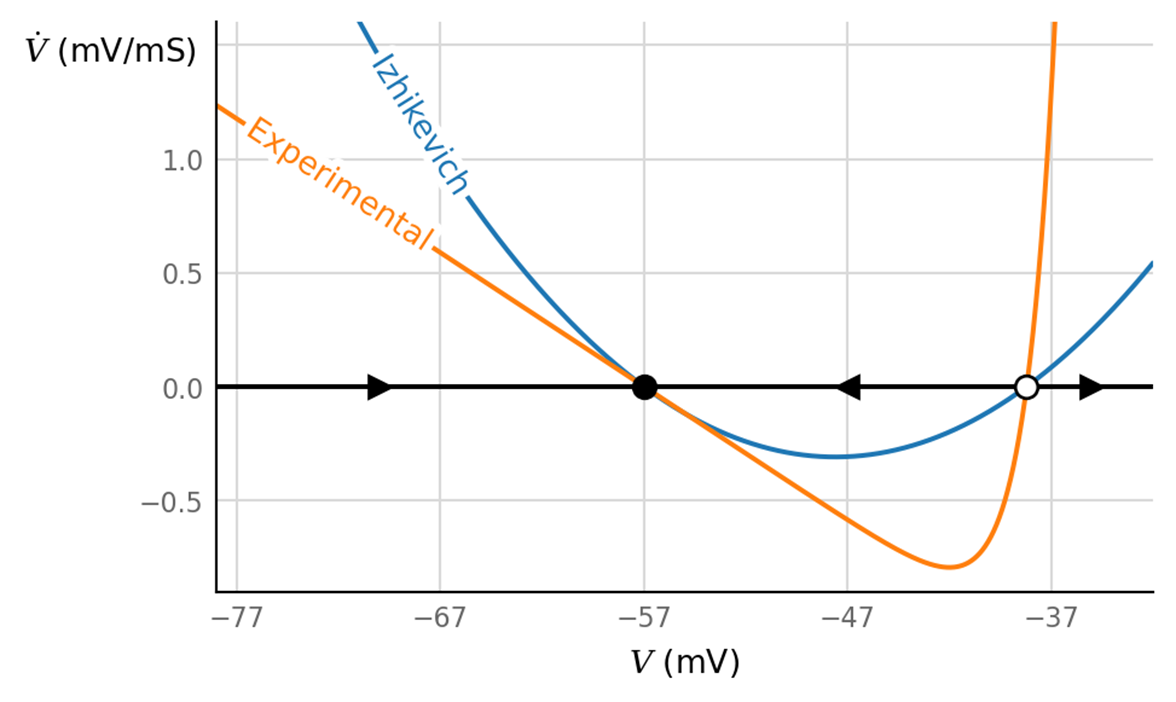
\includegraphics[w=0.9]{dynsys.png}
    \end{sidecaption}
\end{figure}

\section{The Izhikevich neuron}

Another alternative neuron model is the Izhikevich neuron, which is exceedingly similar to the AdEx neuron.
These are the Izhikevich equations, using the same symbols as used before (in \cref{eq:AdEx-V,eq:AdEx-w,eq:AdEx-reset}):
\begin{align}
    C \d{V} &=  k (V - E_L) (V - E_T) - I_\syn - w  \label{eq:Izh-V}  \\[1em]
    τ_w \d{w} &= a (V - E_L) - w     \label{eq:Izh-w} \\[2em]
    \text{if}\ V& > θ,\ \text{then:}  \label{eq:Izh-reset} \\
        &V ← V_r \notag \\
        &w ← w + Δw \notag
\end{align}

We have introduced two new parameters not present in the AdEx equations: the steepness of the parabola, $k$; and $E_T$, the instantaneous firing threshold (the firing threshold in the absence of any synaptic or adaptation currents).

The only difference with AdEx is in \cref{eq:Izh-V}, where the $F(V)$ curve is not made by a linear plus exponential term, as in AdEx; but rather by a quadratic (a parabola). Its two zeros (the fixed points) are readily apparent, as $E_L$ and $E_T$.


\subsection{Correspondences with AdEx}

In Izhikevich's book\footnote{\cite{Izhikevich2007DynamicalSystemsNeuroscience}, section 5.2.4, equations 5.7 \& 5.8}, different names are used for the same quantities:
\begin{align}
    C \d{v} &= k(v - v_r)(v-v_t) - u + I \label{eq:IzhIzh-v} \\[1em]
    \d{u} &= a(b(v-v_r) - u) \\[2em]
    \text{if}&\ v > v_\text{peak},\ \text{then:} \\
    v &← c  \notag \\
    u &← u + d  \notag
\end{align}

\Cref{tab:AdEx-Izh-compar} compares both notation conventions.

\begin{table}[h]
    \begin{sidecaption}
        {Different symbols used for the same quantities in \cite{Naud2008FiringPatternsAdaptive} (`AdEx') and \cite{Izhikevich2007DynamicalSystemsNeuroscience} (`Izh').
        Membrane capacitance $C$ (in farad) is the same in both notations.}
        [tab:AdEx-Izh-compar]
        \begin{tabular}{c c l c}
            AdEx   & Izh  & Description & Units \\
            \hline
            $V$  & $v$   & Membrane voltage & V \\
            $w$  & $u$   & Adaptation current & A \\
            $τ_w$  & $1/a$   & Time constant of adaptation current & s \\
            $E_L$  & $v_r$  & Resting / leak potential & V \\
            $V_r$  & $c$  & Reset voltage after spike & V \\
            $a$  & $b$ & Sensitivity of adapt. current to $V$ & S \\
            $b$  & $d$ & Adaptation current bump after spike & A \\
        \end{tabular}
    \end{sidecaption}
\end{table}

Beside these straightforward correspondences, there are some parameters in either model that have no direct equivalent in the other: $k$ and $v_t$ in Izhikevich, and $g_L$, $Δ_T$, and $V_T$ in AdEx.
For those, we'll look at the shape of Izhikevich's $F(V)$, as we've done for the AdEx neuron before.

First, the AdEx parameter $g_L$. This is the input conductance, a.k.a. the leak conductance, and the slope of $F(V)$ around the leak potential. We can find this same conductance for the Izhikevich neuron by taking the derivative with respect to $v$ of the right hand side of \cref{eq:IzhIzh-v}, at $w = 0$, $I_\syn = 0$, and $v = v_r$. We find:
\begin{equation}
    \dd{v}(k(v-v_r)(v-v_t)) \Big|_{v=v_r} = k(v_r - v_t)
\end{equation}
(this value is negative: the leak potential is a stable fixed point. This corresponds to \cref{eq:AdEx-V}, where we find `$-g_L$').
Thus, our first nontrivial correspondence:
\begin{equation}
    g_L = k (v_t - v_r)  \label{eq:leak_conductance}
\end{equation}

We've seen that $V_T$ is the minimum of AdEx's $F$.
The minimum of Izhikevich's $F$ is easily found as the average of the parabola's two zeros. I.e, $V_T$ corresponds to $(v_r + v_t) / 2$.

Finally, $Δ_T$ co-determines the slope of AdEx's $F$ at the firing threshold (\cref{eq:AdEx-slope}). Given that Izhikevich's $F$ is a parabola, with slopes equal in magnitude at both roots, we already know the firing threshold slope: it is the same as the leak conductance, \cref{eq:leak_conductance}.\\
Here, the AdEx model is more expressive than Izhikevich's: the slope of $\d{V}$ at the firing threshold can be independently tweaked from the leak conductance; in Izhikevich these two are clung together by the form of the quadratic equation.


\subsection{Comparison with AdEx}

The Izhikevich and AdEx models are very similar. Their phase spaces are topologically identical:
the adaptive current equation is identical (up to a renaming of the variables); and the $F(V)$-graph has the same shape, with two fixed points: a stable fixed point at the resting potential, and an unstable one at the firing threshold (\cref{fig:dynsys}).

They differ in the exact shape: Izhikevich's $F(V)$ is a parabola, while AdEx is the more realistic 'linear subthreshold, and then transitioning to an exponential' (see \cref{fig:exIF-fit,fig:dynsys}).
As a result, Izhikevich neurons have an unrealistically slow spike upstroke.

\begin{figure}
    \hspace*{10em}
    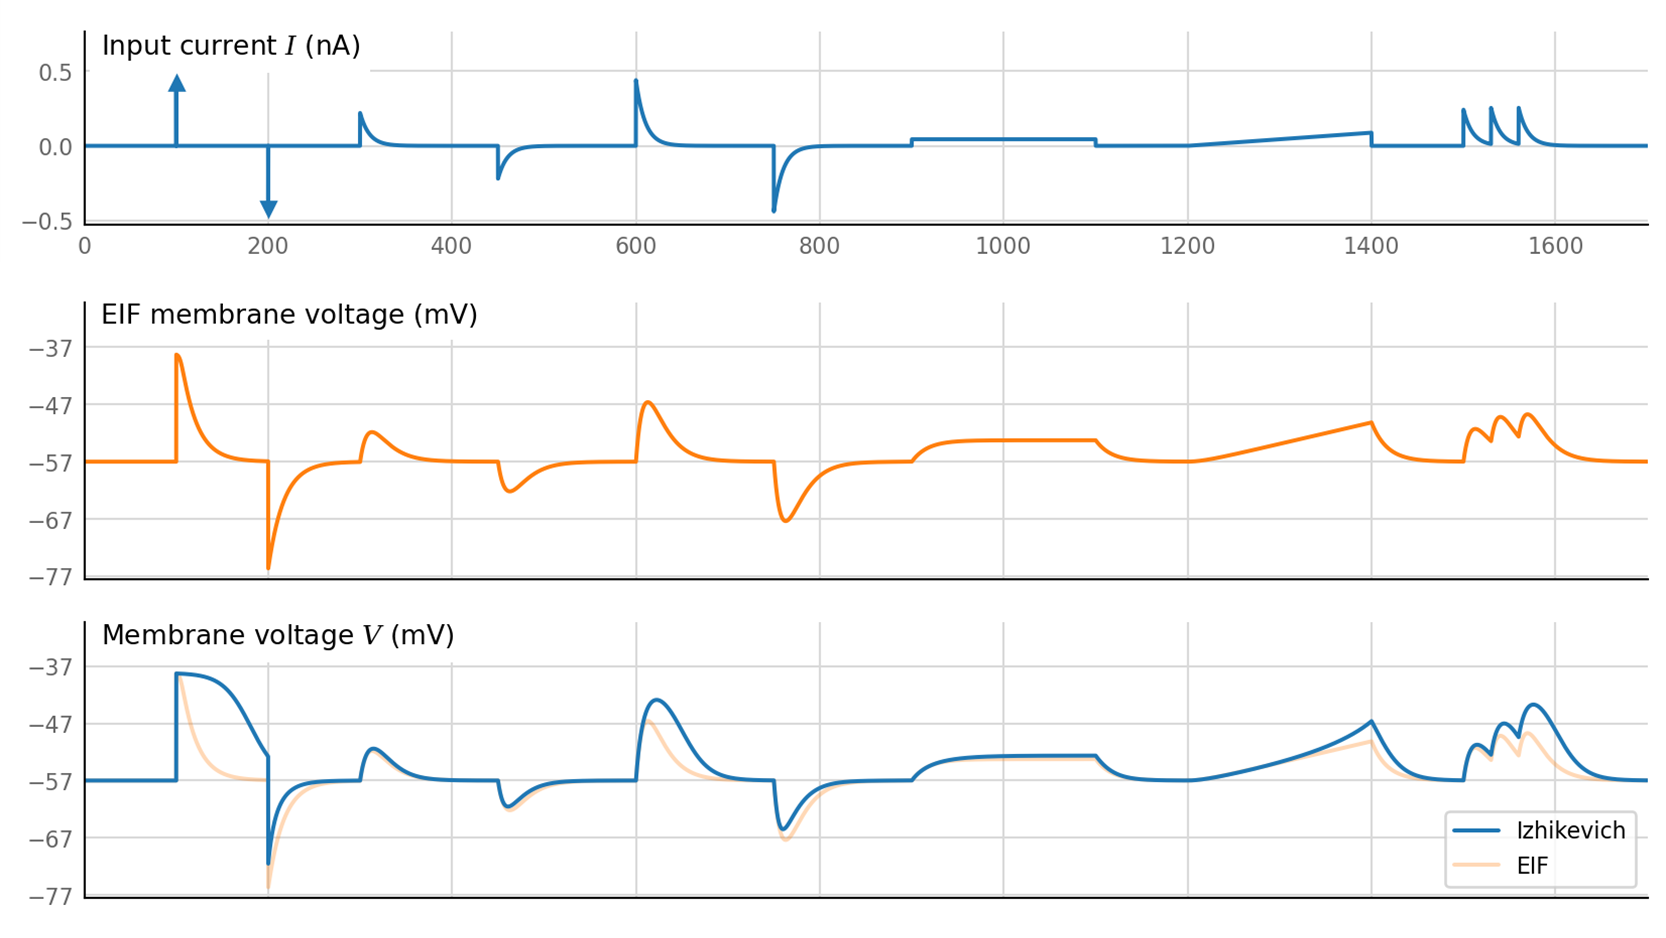
\includegraphics[w=1.5]{testbench-I-Izh-EIF.png}
    \caption{The nonlinear response of Izhikevich neurons to subthreshold input currents. `EIF' stands for exponential integrate-and-fire; it has the same $\d{V}$ as an AdEx neuron. Adaptation currents are negligibly small for both models in this test scenario.
    % Izhikevich parameters from \cite{Izhikevich2007DynamicalSystemsNeuroscience,Humphries2006UnderstandingUsingIzhikevich}, for a Cortical Regular Spiking neuron.
    % EIF parameters chosen to match: $C = 100$ pF, $E_L = -60$ mV, $R = 80\, \si{\mega\ohm}$.
    }
    \label{fig:testbench-I-Izh-EIF}
\end{figure}

A second issue is Izhikevich's subthreshold nonlinearity. The effects of this can be seen in \cref{fig:testbench-I-Izh-EIF}. Positive input currents produce stronger responses than equally large negative input currents. This is explained by the quadratic $\d{V}$ shape: positive deviations are attenuated less, and negative deviations more, than a linear neuron would. Real and AdEx neurons do not suffer this assymetry.

This nonlinearity is not visible for small voltage deviations, which is what the postsynaptic potentials we are interested in in this thesis tend to be. There is however an effect of the neuron's average voltage: if this voltage is constantly on the higher side, then inputs -- both negative and positive -- will cause larger responses than if the median voltage was lower.



\clearpage
\section{Synapse model}
\label{sec:synapse_model}

One unexplained term in our neuron model, \cref{eq:AdEx-V}, is the synaptic current $I_\syn$.
This is the following sum over all input synapses $i$ of the neuron:
\begin{equation}
    I_\syn = \sum_i g_i (V - E_i)
    \label{eq:I_syn}
\end{equation}
where $V$ is the global membrane voltage of the neuron, $E_i$ is the reversal potential of that synapse, and $g_i$ is the local synaptic conductance, which is modulated by presynaptic spikes.

For an excitatory synapse, $V < E_i$, making $g_i (V - E_i)$ negative, increasing the membrane voltage according to the sign convention for $I_\syn$ in \cref{eq:AdEx-V}.

We simulate the synaptic conductances $g_i$ as exponentially decaying signals (with time constant $\tau$), and bump them up instantaneously on arrival of a presynaptic spike:
\begin{gather}
    \d{g_i} = -g_i / \tau
    \label{eq:g_i}
    \\[1em]
    \text{On incoming presynaptic spike:}\notag\\
    \ g_i ← g_i + Δg_i
\end{gather}

\marginpar{
    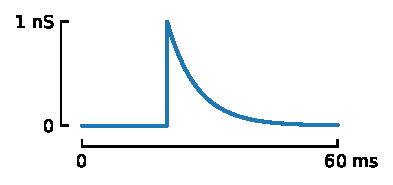
\includegraphics{g1.pdf}
    \captionof{figure}{Example synaptic conductance trace $g_1(t)$, with a single incoming spike at $t = 20$ ms.}
    \label{fig:g1}
}
\marginpar{
    \vspace*{3em}
    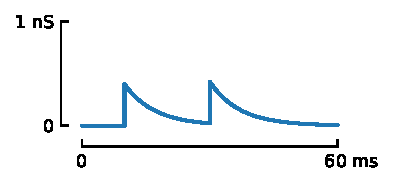
\includegraphics{g2.pdf}
    \captionof{figure}{Another example trace $g_2(t)$, with spikes at $t = 10$ ms and $30$ ms, and a smaller $Δg$.}
    \label{fig:g2}
}

Note that these are not the so called alpha-synapses. Those are two dimensional and also have an exponential rise, instead of just an exponential decay. (For an infinitely fast rise though, these models are of course the same).
Simulating a full alpha synapse might increase the realism of our voltage traces, for a small simulation cost. We did not try this however. Foremost because alpha synapses fit to real data often have very fast rise times that are almost indistinguishable from instantaneous jumps.

For efficiency, we give all our excitatory synapses the same reversal potential, $E_\exc$. Idem for the inhibitory synapses, with $E_\inh$. This allows us to factor the synaptic current sum (\cref{eq:I_syn}) as follows:
\begin{equation}
    I_\syn = (V - E_\exc) \sum_{\exc\ i} g_i \  + \  (V - E_\inh) \sum_{\inh\ i} g_i
    \label{eq:I_syn_factor}
\end{equation}

The sums of conductance signals $g_i(t)$ can also be simplified. Say that the values of $g_i$ at $t = 0$ are $G_i$. The solution to \cref{eq:g_i} (at least in the time until a new presynaptic spike arrives) is then
\begin{equation}
    g_i(t) = G_i\ e^{-t/\tau}
\end{equation}

With this, and when all synapses have the same time constant $\tau$, the two sums in \cref{eq:I_syn_factor} can be factored as follows:\footnotemark
\footnotetext{
    This is only valid in the time before any new spikes arrive.
    But the `summability' still holds after a new spike.
    To see this, the given reasoning can be repeated, but simply with different values for the $G_i$ (all decayed by an amount $e^{-t_\text{spike}/\tau}$, and one increased by a bump $Δg_i$), and then redefining $t_\text{spike}$ to be $t = 0$.
}
\begin{equation}
    \sum_i g_i(t) = \sum_i \left( G_i\ e^{-t/\tau} \right)
                            = \left( \sum_i G_i  \right) e^{-t/\tau}
\end{equation}
This means that we need to only keep track of two conductance signals: $g_\exc$ and $g_\inh$, each the sum of all excitatory or all inhibitory synaptic conductances.

\marginpar{
    \vspace*{2em}
    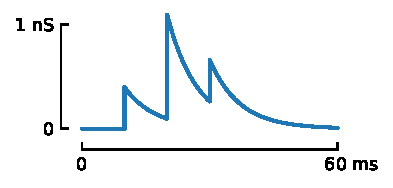
\includegraphics{g3.pdf}
    \captionof{figure}{A third synaptic conductance trace $g_3(t)$, with three input spikes at the same times and strengths as in \cref{fig:g1,fig:g2}. This signal is simulated independently, but turns out to be equal to the sum of the two others: $g_3(t) ≡ g_1(t) + g_2(t)$.}
}

Our synaptic current sum then becomes simply:
\begin{equation}
    I_\syn = (V - E_\exc)\ g_\exc \  + \  (V - E_\inh)\ g_\inh,
\end{equation}
and we only need to simulate two differential equations, instead of one for every synapse:
\begin{align*}
    \d{g_\exc} &= -g_\exc / \tau \\
    \d{g_\inh} &= -g_\inh / \tau,
\end{align*}
where on arrival of a spike at synapse $i$ either $g_\exc$ or $g_\inh$ is instantaneously increased by a value $Δg_i$, depending on whether that synapse is excitatory or inhibitory.


\section{Input spikes}

In our simplest experimental setup, we simulate just one AdEx neuron.
Its input is provided by an array of $N$ Poisson neurons, i.e. they each generate spike trains according to a Poisson process. We call this the `N-to-1' setup.

The inter-event intervals of a Poisson process follow an exponential distribution.
We use that fact to generate spike trains: we draw samples from $\mathrm{Exp}(\lambda)$ (with $\lambda$ the desired firing rate), and cumulatively sum up these intervals  to obtain spike times. This is done until we have reached the desired input train duration.


\section{Voltage imaging}

The signals detected by a light microscope in a voltage imaging setup are not the same as the real membrane voltage signals of which they are a reflection.

We model this lossy transformation by simply adding Gaussian noise to our simulated membrane voltage. As in the voltage imaging literature, we quantify the amount of this  noise by a `spike-SNR' measure (spike signal-to-noise ratio). This is defined as the height of an average spike relative to the standard deviation of the noise.

A more realistic model of the voltage-imaging transformation would also incorporate the exponential decay over time of the SNR, and the short-term 'smearing in time' of voltage indicators. The latter could be done by passing the voltage signal through a linear filter with some non-instantaneous impulse response.
